\documentclass[11pt]{article}
\usepackage{lmodern}
\usepackage[margin=1in]{geometry}
\usepackage{graphicx, amsmath, amsthm}
% \renewcommand*\rmdefault{cmdh}
% \usepackage[T1]{fontenc}

\title{Term Paper on Johannas Kepler \\
\small Differential Equations \\
University of Massachusetts Lowell \\
Summer 2020}
\author{Joel Savitz}

\begin{document}
% \normalfont
\maketitle

\section{Abstract}

Johannes Kepler is a widely known name
in mathematical and scientific history.
In this paper, I explore his origins
and early scientific mindset,
then I give a general overview of
his early to mid stage academic career,
and finally I provide some examples
of his more significant contributions
to science and discuss his resulting legacy.

\section{Early life}

Johannes Kepler was born in the Holy Roman Empire in 1571.
Despite his father leaving the family when he was five
as well as premature birth, 
he is said to have impressed visitors at his
grandfathers' inn with his mathematical prowess
from an early age \cite{caspar}.
In Kepler's own words,
his love for astronomy began at the age of six
when he ``was taken by [his] mother to a high place to look at"
the great comet of 1577, observing that
it ``appeared quite red" \cite{koestler}.


After being introduced to Copernican heliocentrism
in his study at the University of Tübingen,
Kepler defended this position
--- theologically and technically --
in a student disputation \cite{westman}.
His skill as an astronomer as well as
his unusually strong mathematical ability
led him to an acedemic appointment
as a teacher of mathematics and astronomy
at the University of Graz in 1594
at the age of 23,
beginning a long and successful academic career \cite{caspar}.

\section{Academic career}

Starting off his tenure with a bang,
Kepler was the first to publish a defense
of Copernican heliocentrism.
This early work,
entitled \textit{Mysterium Cosmographicum},
attempted to describe
the arrangement of the solar system
in terms of inscribed platonic solids,
though he later rejected this formulation \cite{caspar}.
Fundamentally, Kepler was driven by religious zeal.
His model of the universe was as an image of God
and his work connected Christian spiritual concepts
with astronomical phenomena.
An early draft of the work
extensively defended heliocentrism
using textual evidence from the bible itself \cite{barker}.

Kepler spent the next few years at Graz
doing research with the goal of extending
and elaborating on his first work,
but extensive correspondence with Tycho Brahe
--- a great figure in astronomy and a contemporary of Kepler ---
convinced Kepler
of the inconsistency and inaccuracy
of some of his beliefs, 
so Kepler instead studied the relationship between
music, mathematics, and physics,
creating new elaborate theories,
but frustration with
the inaccuracy of existing experimental data
as well as the invitation of Brahe
led Kepler to relocate to leave Graz
on New Year's Day 1600 \cite{caspar}.

Before arriving in Prague,
Kepler was a guest of Brahe
and he pursued formal employment,
but negotiations broke down
and Kepler soon moved
with his family to Prague,
due in no small part to their
banishment from Graz
because of their refusal
to convert to Catholicism.
When Brahe passed unexpectedly in October 1601,
Kepler was chosen to succeed him
as the imperial mathematician
for the Holy Roman Emperor
and he was tasked with
continuing where Brahe left off.
His 11 year tenure in this role
is considered to be the
most productive period of Kepler's life \cite{caspar}.

One evening in October 1604,
a supernova occurred in space
that was visible from the earth.
After initially refusing to believe the rumors,
Kepler soon commenced a systematic
observation of the phenomenon.
His role as imperial mathematician
required the interpretation of this
event through an astrological perspective,
but he also made the observation
that the star was fading,
undermining the at the time unquestioned
Aristotelian dogma of the immutability of the heavens \cite{caspar}

% \begin{itemize}
% 	\item Supernova of 1604
% 	\item Advisor to Holy Roman Emperor
% \end{itemize}

\section{Contributions to Physics and Mathematics}

Over the course of his 58 year lifetime,
Kepler made many important contributions
to the fields of mathematics and physics.
In a pamphlet to a friend for a New Year's gift,
he stated what we now refer to as the Kepler conjecture,
the proposition
``that no arrangement of equally sized spheres
filling space has a greater average density than
that of the cubic close packing (face-centered cubic)
and hexagonal close packing arrangements" \cite{conjecture}.
The journal \textit{Forum of Mathematics, Pi}
accepted and published a formal proof
of the Kepler conjecture
authored by a team led by Thomas Hales in 2017,
establishing the Kepler conjecture
as a mathematical theorem.
Hales et al. leveraged the power of
the software proof assistants HOL Light and Isabelle \cite{hales},
utilizing modern automated computational systems
to produce previously elusive solutions to ancient questions.

One of the most influential works
Kepler published was \textit{Astronomiae Pars Optica}
-- The Optical Part of Astronomy ---
inspired by his earlier study of the moon.
In this text,
he described the inverse square law
that describes the intensity of light and reflection
and the sizes of the celestial objects.
In addition,
many neuroscientists agree that
in this text
he was the first to recognize
that light entering the human eye 
forms an inverted and reversed image on the retina \cite{finger}.
He also proposed many
fundamental ideas of projective geometry,
relating to conic sections,
straight lines with infinite length,
and continuous change.
\textit{Astronomiae Pars Optica} is widely considered
to be one of the foundational texts of modern optics \cite{caspar}.



% \begin{itemize}
% 	\item Biblical chronology and astrology
% 	\item Harmonices Mundi
% 	\item Rudolphine Tables
% \end{itemize}

\section{Legacy}

\begin{figure}
\centering
	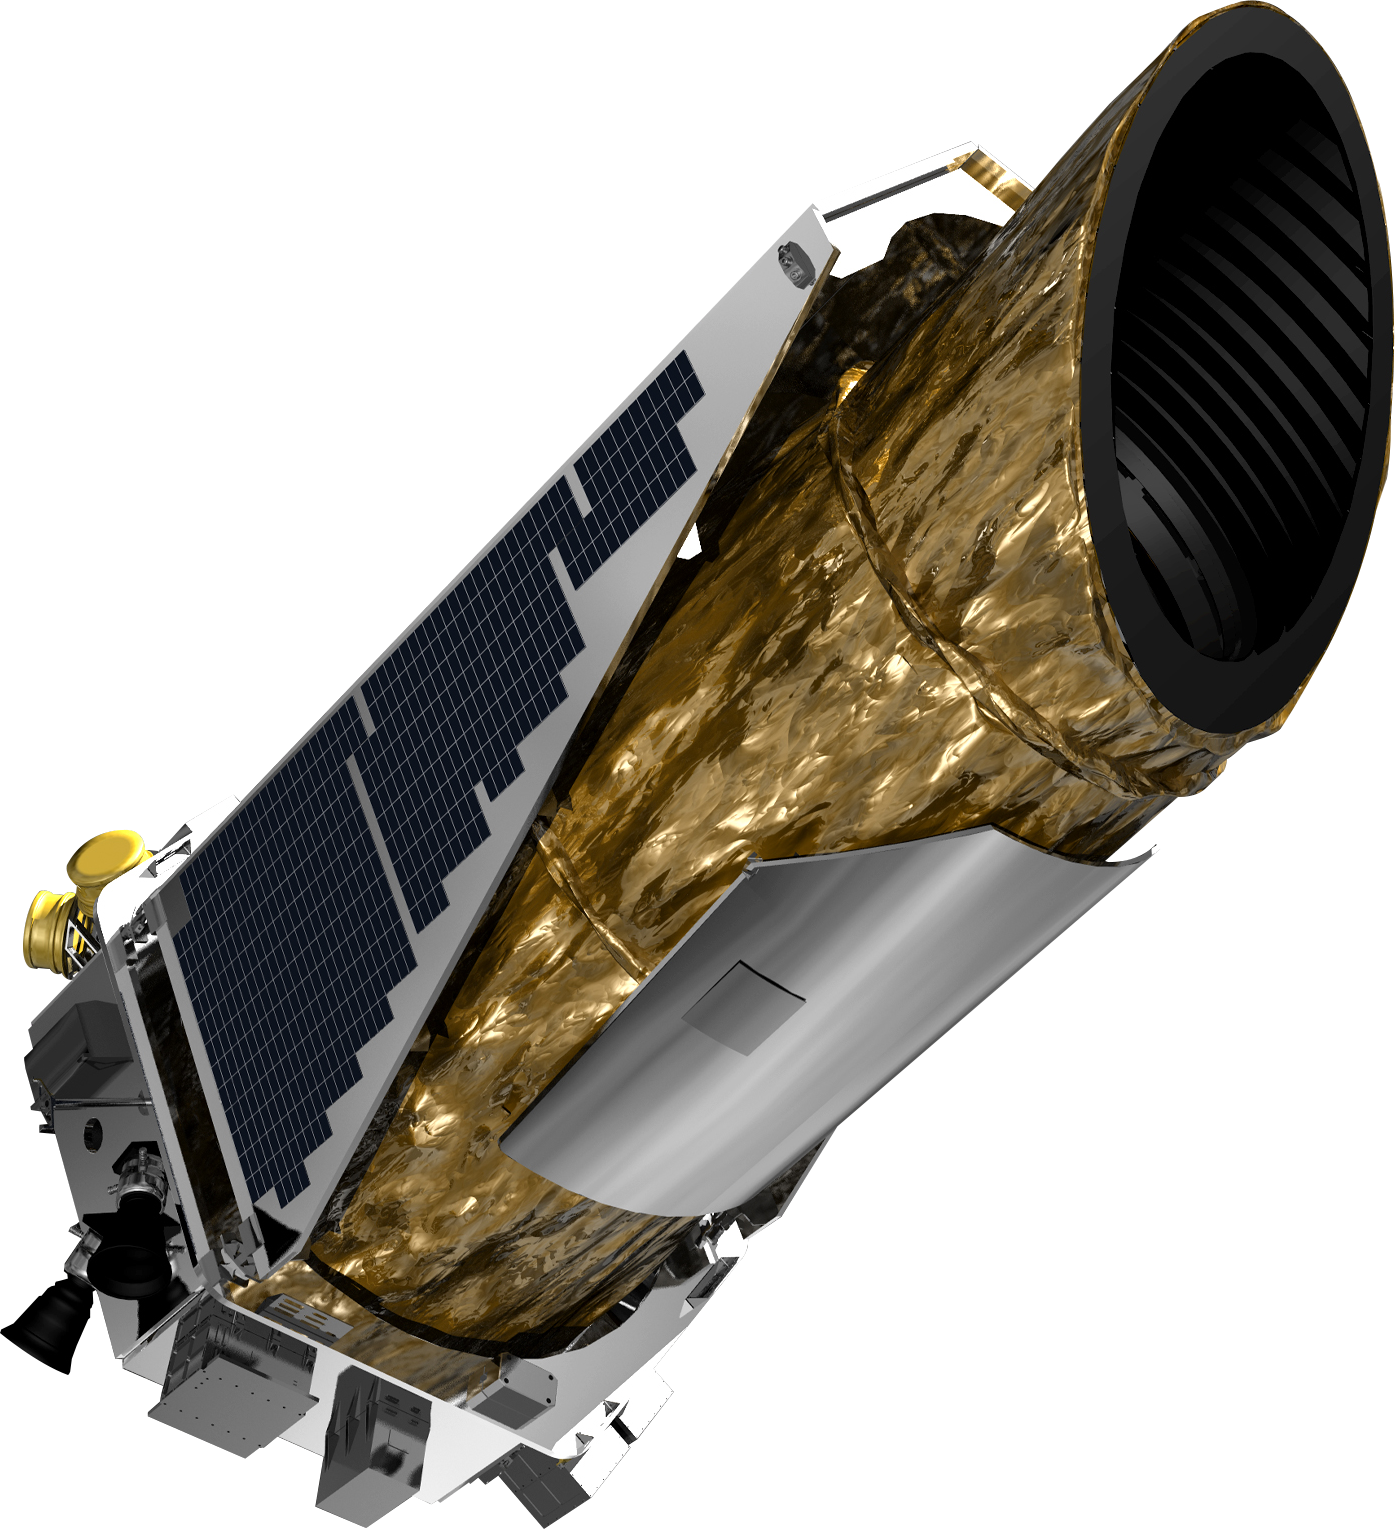
\includegraphics[scale=0.7]{kepler_telescope.png}
	\caption{An artist's depiction of the Kepler space telescope \cite{telpic}}
\label{kepler_telescope}
\end{figure}

Johannes Kepler lives on as his
successors stand on his shoulders
and the shoulders of giants like him.
He was instrumental in the development of
a variety of scientific fields including
astronomy, physics, mathematics, and optics.
A number of scientific ideas are named after Kepler,
including Kepler's laws of planetary motion,
Kepler's Supernova,
and of course the Kepler space telescope,
depicted in figure \ref{kepler_telescope}.
Kepler remains  a household name in
scientifically literate communities
throughout the world.

\bibliographystyle{acm}

\bibliography{paper.bib}

\end{document}
